\documentclass[11pt, oneside]{article}   	% use "amsart" instead of "article" for AMSLaTeX format
\usepackage{geometry}                		% See geometry.pdf to learn the layout options. There are lots.
\geometry{letterpaper}                   		% ... or a4paper or a5paper or ... 
%\geometry{landscape}                		% Activate for for rotated page geometry
%\usepackage[parfill]{parskip}    		% Activate to begin paragraphs with an empty line rather than an indent
\usepackage{graphicx}				% Use pdf, png, jpg, or eps� with pdflatex; use eps in DVI mode
								% TeX will automatically convert eps --> pdf in pdflatex		
\usepackage{amssymb}
\usepackage{amsmath}

\title{Plane and a point}
%\author{The Author}
%\section{}
% \subsection*{R code}
\date{}							% Activate to display a given date or no date

\graphicspath{{/Users/telliott_admin/Dropbox/Tex/png/}}

% \begin{center} 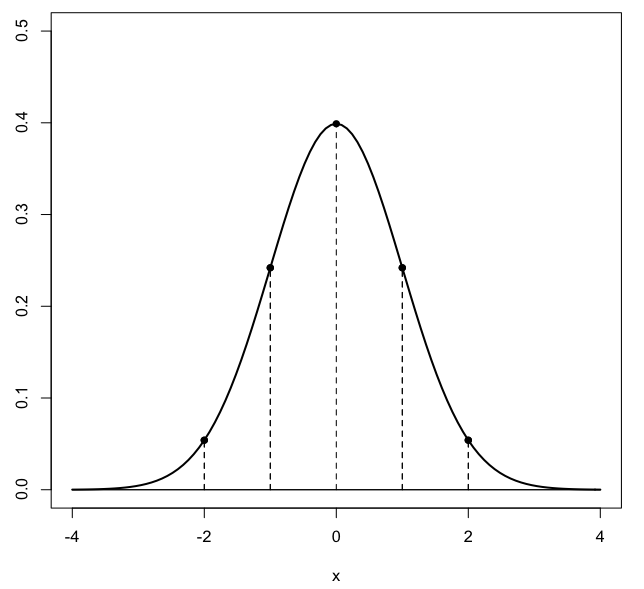
\includegraphics [scale=0.4] {gauss3.png} \end{center}
% \begin{bmatrix} a  &  b \\ c  &  d \end{bmatrix}
\begin{document}
\maketitle
\large
%\noindent

Consider the plane containing three points $(1,0,0)$, $(0,1,0)$, and $(0,0,1)$.  Find two vectors in the plane by subtracting the second and third from the first.
\[ u = (1,0,0) - (0,1,0) =  \ <1,-1,0> \]
\[ v = (1,0,0) - (0,0,1) = \ <1,0,-1> \]
Obtain the normal vector by computing the cross product
\[ N = u \times v 
\Rightarrow 
\begin{vmatrix}
i & j & k \\
1 & -1 & 0 \\
1 & 0 & -1 \\ 
\end{vmatrix} 
= 1i + 1j + 1k = \ <1,1,1>  \]
One equation of the plane is then
\[ N \cdot w = 0 \] 
for any vector $w$ in the plane.
\vspace{5 mm}

\noindent
Consider a fixed point in the plane ($x_0,y_0,z_0$).  Then any other point in the plane $(x,y,z)$ yields a vector from the fixed point which, dotted with $n$, yields $0$
\[ \ <x-x_0,y-y_0,z-z_0> \  \cdot \ <1,1,1> \ = 0 \]
\[ x - x_0 + y - y_0 + z - z_0 = 0 \]
\[ x + y + z = x_0 + y_0 + z_0 = d \]
Plugging in one of the points yields
\[ x + y + z = 1 \]
\vspace{5 mm}

\noindent
Consider any point in space, e.g. $P = (3,4,6)$.  Find the point $Q$ on the plane which is closest to $P$, the point we arrive at by subtracting some fraction of $N$ from $P$.  We have a point and a vector
\[ Q = P - tN \]
\[ Q = (3,4,6) \ - \ t <1,1,1> \ \]
Since $Q$ is in the plane, its components $x,y,z$ satisfy $x + y + z = 1$!  So
\[ (3-t) + (4-t) + (6-t) = 1 \]
\[ 13 -3t = 1\]
\[ t = 4 \]
\[ Q = (-1,0,2) \]
Check that $Q$ is in the plane
\[ -1 + 0 + 2 = 1 \]
and $P-Q$ is parallel to $N$
\[ P - Q = \ <4,4,4> \]
which is definitely a multiple of $N$.  
\vspace{5 mm}

\noindent
Where does the vector $w$ that goes from the origin to point $P=(3,4,6)$ hit the plane?  Call that point $R$.  Again we have a point and a vector 
\[ R = (0,0,0) + tw = (0,0,0) + t<3,4,6> \]
And again, since $R$ is in the plane, its components $x,y,z$ satisfy $x + y + z = 1$.  So
\[ 3t + 4t + 6t = 1 \]
\[ t = \frac{1}{13} \]
\[ R = (\frac{3}{13}, \frac{4}{13}, \frac{6}{13}) \]
Notice that the vector $Q-R$ is in the plane, as it should be
\[ (Q-R) \cdot N =  ((-1,0,2) - (\frac{3}{13}, \frac{4}{13}, \frac{6}{13})) \cdot \ <1,1,1> \ \]
\[ =  \ <\frac{-16}{13}, \frac{-4}{13}, \frac{20}{13}> \  \cdot  \ <1,1,1>  \ = 0 \]
And, adding the horizontal and vertical components together
\[ Q - R + P - Q = P - R = (3,4,6) - (\frac{3}{13}, \frac{4}{13}, \frac{6}{13}) \]
\[ = (\frac{36}{13}, \frac{48}{13}, \frac{72}{13}) \]
the result is parallel to $w$.






\end{document}  